%% ============================================================
%%  SECCIÓN 13 — Anexos
%% ============================================================

\begin{appendices}

\section{Deducción analítica formal de las ecuaciones de carga y descarga}
\label{sec:anexo_deducciones}

\subsection{Proceso de carga con fuente constante mediante transformada de Laplace}

En la Sección~\ref{sec:fundamento} se resolvió la ecuación diferencial del circuito RC en el dominio del tiempo mediante separación de variables. Para fundamentar el análisis desde la perspectiva de sistemas lineales e invariantes en el tiempo (LTI) de la teoría de control y telecomunicaciones, presentamos a continuación la deducción empleando la transformada de Laplace \cite{alexander}.

Consideremos la ecuación íntegro-diferencial de la malla en reposo ($q(0^-) = 0$):
\begin{equation}
    R\,i(t) + \frac{1}{C}\int_{0^-}^{t} i(\lambda)\,d\lambda = V_0 \cdot u(t)
    \label{eq:malla_laplace}
\end{equation}
donde $u(t)$ es la función escalón unitario de Heaviside. Aplicando la transformada unilateral de Laplace ($\mathcal{L}\{f(t)\} = F(s)$):
\begin{equation}
    R\,I(s) + \frac{1}{s C}\,I(s) = \frac{V_0}{s}
\end{equation}
Factorizando la intensidad de corriente en el plano complejo de frecuencias $s$:
\begin{equation}
    I(s)\left( R + \frac{1}{s C} \right) = \frac{V_0}{s} \implies I(s)\left( \frac{s R C + 1}{s C} \right) = \frac{V_0}{s}
\end{equation}
Despejando $I(s)$:
\begin{equation}
    I(s) = \frac{V_0\,C}{s R C + 1} = \frac{V_0 / R}{s + \frac{1}{R C}}
\end{equation}
Aplicando la transformada inversa de Laplace ($\mathcal{L}^{-1}\{(s + a)^{-1}\} = e^{-a t}$):
\begin{equation}
    \boxed{i(t) = \frac{V_0}{R}\,e^{-t / RC} \cdot u(t)}
\end{equation}
Para la diferencia de potencial en bornes del condensador $V_C(s)$:
\begin{equation}
    V_C(s) = \frac{1}{s C}\,I(s) = \frac{V_0 / (R C)}{s\left(s + \frac{1}{R C}\right)}
\end{equation}
Descomponiendo en fracciones simples:
\begin{equation}
    \frac{V_0 / (R C)}{s\left(s + \frac{1}{R C}\right)} = \frac{A}{s} + \frac{B}{s + \frac{1}{R C}} \implies A = V_0, \quad B = -V_0
\end{equation}
Por consiguiente:
\begin{equation}
    V_C(s) = \frac{V_0}{s} - \frac{V_0}{s + \frac{1}{R C}}
\end{equation}
Antitransformando al dominio del tiempo:
\begin{equation}
    \boxed{v_C(t) = V_0 \left( 1 - e^{-t / RC} \right) u(t)}
\end{equation}
lo que demuestra con absoluta generalidad matemática la forma de onda exponencial observada en el osciloscopio.

\subsection{Proceso de descarga libre del condensador}

Para la descarga libre, considerando como condición inicial $v_C(0) = V_0$ y fuente nula ($V_0 = 0$):
\begin{equation}
    R\,I(s) + \frac{1}{s C}\left( I(s) + C V_0 \right) = 0 \implies I(s)\left( R + \frac{1}{s C} \right) = -\frac{V_0}{s}
\end{equation}
\begin{equation}
    I(s) = -\frac{V_0 / R}{s + \frac{1}{R C}} \implies \boxed{i(t) = -\frac{V_0}{R}\,e^{-t / RC}}
\end{equation}
\begin{equation}
    V_C(s) = \frac{I(s) + C V_0}{s C} = \frac{V_0}{s + \frac{1}{R C}} \implies \boxed{v_C(t) = V_0\,e^{-t / RC}}
\end{equation}

\section{Propagación analítica de incertidumbres metrológicas (Norma GUM)}
\label{sec:anexo_propagacion}

A partir de la función de medición de capacitancia:
\begin{equation}
    C = f(\tau, R) = \frac{\tau}{R}
\end{equation}
los coeficientes de sensibilidad metrológica corresponden a los gradientes locales de la función:
\begin{equation}
    c_\tau = \frac{\partial f}{\partial \tau} = \frac{1}{R}, \qquad c_R = \frac{\partial f}{\partial R} = -\frac{\tau}{R^2}
\end{equation}
Bajo la hipótesis de magnitudes de entrada no correlacionadas, la varianza combinada resulta:
\begin{equation}
    u_c^2(C) = c_\tau^2\,u^2(\tau) + c_R^2\,u^2(R) = \left( \frac{1}{R} \right)^2 u^2(\tau) + \left( -\frac{\tau}{R^2} \right)^2 u^2(R)
\end{equation}
Dividiendo la varianza combinada entre $C^2 = (\tau / R)^2$, obtenemos la suma en cuadratura de las incertidumbres relativas:
\begin{equation}
    \left( \frac{u_c(C)}{C} \right)^2 = \left( \frac{u(\tau)}{\tau} \right)^2 + \left( \frac{u(R)}{R} \right)^2
\end{equation}
Extrayendo la raíz cuadrada y aplicando el factor de cobertura $k=2$:
\begin{equation}
    \boxed{U(C) = 2 \cdot C \cdot \sqrt{\left(\frac{u(\tau)}{\tau}\right)^2 + \left(\frac{u(R)}{R}\right)^2}}
    \label{eq:anexo_gum_recuadro}
\end{equation}
Sustituyendo los valores globales obtenidos por el método de regresión lineal para los tres condensadores de la Mesa C7:
\begin{gather}
    \boxed{C_1 = \qty{10,79 \pm 0,05}{\nano\farad} \quad (k=1; \text{ error rel. } \qty{+7,95}{\percent})} \\
    \boxed{C_2 = \qty{27,44 \pm 0,03}{\nano\farad} \quad (k=1; \text{ error rel. } \qty{+22,48}{\percent})} \\
    \boxed{C_3 = \qty{34,61 \pm 0,29}{\nano\farad} \quad (k=1; \text{ error rel. } \qty{+4,15}{\percent})}
\end{gather}

\section{Resolución exhaustiva del cuestionario oficial de la guía}
\label{sec:anexo_cuestionario}

A continuación se presentan las respuestas analíticas y experimentales completas a cada una de las interrogantes formuladas en la guía oficial de laboratorio.

\subsection{Pregunta a) del cuestionario oficial}
\begin{quote}
    \textit{«¿Podría usar una frecuencia de \qty{100}{\kilo\hertz} en lugar de \qty{250}{\hertz} para hallar el tiempo $\tau = RC$ de los circuitos RC que usted ha analizado en este experimento? ¿Por qué?»}
\end{quote}

\textbf{Respuesta:} \textbf{NO es físicamente posible} utilizar una frecuencia de \qty{100}{\kilo\hertz} para determinar la constante de tiempo $\tau$ con los componentes asignados a nuestro banco de trabajo.

\textbf{Demostración cuantitativa:}
\begin{enumerate}
    \item \textbf{Condición operativa real a $f = \qty{250}{\hertz}$:}
    \begin{itemize}
        \item El período de la señal es $T = 1 / \qty{250}{\hertz} = \qty{4,00}{\milli\second} = \qty{4000}{\micro\second}$.
        \item El semiperíodo disponible para que el condensador cargue o descargue es:
        \begin{equation*}
            \frac{T}{2} = \qty{2,00}{\milli\second} = \qty{2000}{\micro\second}
        \end{equation*}
        \item En nuestra Mesa C7, las constantes de tiempo registradas oscilaron entre:
        \begin{equation*}
            \tau_{\min} = \qty{24,4}{\micro\second} \quad (R_3 C_1) \qquad \text{y} \qquad \tau_{\max} = \qty{344,8}{\micro\second} \quad (R_1 C_3)
        \end{equation*}
        \item Evaluando para la constante de tiempo más lenta ($\tau_{\max} = \qty{344,8}{\micro\second}$):
        \begin{equation*}
            5\tau_{\max} = 5 \times \qty{344,8}{\micro\second} = \qty{1724}{\micro\second} < \qty{2000}{\micro\second} = \frac{T}{2}
        \end{equation*}
        La relación es $\frac{T/2}{\tau_{\max}} = \frac{2000}{344{,}8} \approx 5{,}8$. Esto garantiza que en cada semiperíodo la curva alcance la meseta asintótica horizontal de saturación completa (\qty{99,7}{\percent} de $V_0$), lo que permite identificar de forma inequívoca el nivel del \qty{100}{\percent} ($V_0 = \qty{10,0}{\volt}$) en el osciloscopio y ubicar con exactitud el nivel del \qty{63,2}{\percent} (\qty{6,32}{\volt}) para medir $\tau$.
    \end{itemize}
    
    \item \textbf{Comportamiento hipotético si la frecuencia se elevara a $f = \qty{100}{\kilo\hertz}$:}
    \begin{itemize}
        \item El período se reduciría drásticamente a $T = 1 / (\qty{100e3}{\hertz}) = \qty{10}{\micro\second}$, con lo cual el semiperíodo de carga duraría únicamente:
        \begin{equation*}
            \frac{T}{2} = \qty{5}{\micro\second}
        \end{equation*}
        \item Comparando este lapso con las constantes de tiempo del circuito:
        \begin{itemize}
            \item Para la constante más rápida ($\tau_{\min} = \qty{24,4}{\micro\second}$):
            \begin{equation*}
                \frac{T/2}{\tau_{\min}} = \frac{\qty{5}{\micro\second}}{\qty{24,4}{\micro\second}} \approx 0{,}205\tau
            \end{equation*}
            Al cabo de $0{,}205\tau$, la tensión en el capacitor apenas alcanzaría:
            \begin{equation*}
                V_C = V_0 \left( 1 - e^{-0{,}205} \right) \approx 0{,}185\,V_0 \implies \qty{18,5}{\percent} \text{ de } V_0
            \end{equation*}
            antes de ser forzado a conmutar hacia la descarga.
            \item Para la constante más lenta ($\tau_{\max} = \qty{344,8}{\micro\second}$):
            \begin{equation*}
                \frac{T/2}{\tau_{\max}} = \frac{\qty{5}{\micro\second}}{\qty{344,8}{\micro\second}} \approx 0{,}0145\tau
            \end{equation*}
            En ese ínfimo lapso, el condensador solo alcanzaría el $1 - e^{-0{,}0145} \approx \qty{1,44}{\percent}$ de $V_0$ (apenas \qty{144}{\milli\volt}).
        \end{itemize}
    \end{itemize}
    \item \textbf{Consecuencia en la pantalla del osciloscopio:} La señal en bornes del condensador degeneraría en una diminuta onda triangular casi imperceptible. Al no formarse jamás una meseta horizontal asintótica, resulta físicamente imposible saber cuál sería la tensión de saturación $V_0$, haciendo inviable fijar la cota del \qty{63,2}{\percent} y medir la constante de tiempo $\tau$.
\end{enumerate}

\subsection{Pregunta b) del cuestionario oficial}
\begin{quote}
    \textit{«Escriba los valores de $R_1$, $R_2$ y $C$ usados en el ítem (t) de procedimientos.»}
\end{quote}

\textbf{Respuesta:} En el montaje experimental del ítem (t) (paso 20 / Figuras 9 y 10 de la guía), se utilizaron los componentes del banco de la Mesa C7:
\begin{itemize}
    \item \textbf{Resistencia en serie $R_1$:}
    \begin{equation*}
        R_1 = \qty{9,980 \pm 0,058}{\kilo\ohm} = \qty{9980}{\ohm} \quad (\text{nominal de catálogo: } \qty{10}{\kilo\ohm})
    \end{equation*}
    \item \textbf{Resistencia en derivación paralelo $R_2$:}
    \begin{equation*}
        R_2 = \qty{6,832 \pm 0,033}{\kilo\ohm} = \qty{6832}{\ohm} \quad (\text{nominal de catálogo: } \qty{6,8}{\kilo\ohm})
    \end{equation*}
    \item \textbf{Condensador $C$ (Condensador $C_3$ del módulo):} Valor rotulado nominal de \qty{33,23}{\nano\farad} y valor efectivo determinado por MCO:
    \begin{equation*}
        C = \qty{34,61 \pm 0,29}{\nano\farad}
    \end{equation*}
    \item \textbf{Señal de entrada:} Onda periódica cuadrada de amplitud $V_0 = \qty{10,0}{\voltpp}$ y frecuencia $f = \qty{250}{\hertz}$.
\end{itemize}

\subsection{Pregunta c) del cuestionario oficial}
\begin{quote}
    \textit{«¿Cuáles son los valores de corriente mínima y máxima durante la carga del condensador que usted observa en el paso 20 del procedimiento? Según sus cálculos, ¿Cuáles deberían ser esos valores?»}
\end{quote}

\textbf{Respuesta y desarrollo analítico:}
En el circuito del paso 20, la fuente escalón conmuta a $V_0 = \qty{10,0}{\volt}$ en $t = 0$.

1. \textbf{Valores teóricos calculados:}
\begin{itemize}
    \item \textbf{Corriente máxima de carga ($t = 0^+$):}
    Al encontrarse el condensador inicialmente descargado ($v_C(0^+) = 0$), actúa como un cortocircuito ideal derivando toda la corriente a tierra. La resistencia $R_2$ queda en paralelo con un cortocircuito, por lo que la corriente que la atraviesa es nula ($I_{R2}(0^+) = 0$). Toda la corriente fluye por $R_1$ y penetra directamente en el condensador:
    \begin{equation*}
        I_{\text{carga},\max} = \frac{V_0}{R_1} = \frac{\qty{10,0}{\volt}}{\qty{9980}{\ohm}} = 1{,}002 \times 10^{-3}\ \unit{\ampere} \approx \mathbf{\qty{1,00}{\milli\ampere}}
    \end{equation*}
    
    \item \textbf{Corriente mínima de carga ($t \to T/2 = \qty{2,00}{\milli\second}$):}
    Dado que la constante de tiempo de Thévenin es $\tau_{\text{th}} \approx \qty{140,1}{\micro\second}$, transcurridos \qty{2000}{\micro\second} se han completado más de $14\tau_{\text{th}}$. El condensador alcanza su estado estacionario permanente y cesa de absorber corriente ($I_C(\infty) = 0$). La corriente total suministrada por la fuente circula exclusivamente a través de la conexión serie formada por $R_1$ y $R_2$:
    \begin{equation*}
        I_{\text{total},\min} = \frac{V_0}{R_1 + R_2} = \frac{\qty{10,0}{\volt}}{\qty{9980}{\ohm} + \qty{6832}{\ohm}} = \frac{\qty{10,0}{\volt}}{\qty{16812}{\ohm}} \approx 0{,}5948 \times 10^{-3}\ \unit{\ampere} \approx \mathbf{\qty{0,59}{\milli\ampere}}
    \end{equation*}
    \textit{(Nota: Si se evalúa estrictamente la rama del capacitor, la corriente mínima es $I_{C,\min} = \qty{0,00}{\milli\ampere}$)}.
\end{itemize}

2. \textbf{Valores observados experimentalmente en el osciloscopio:}
\begin{itemize}
    \item La caída de tensión en bornes de $R_1$ capturada en el Canal 2 mostró un pico instantáneo inicial de:
    \begin{equation*}
        V_{R1}(0^+) \approx \qty{10,0}{\volt} \implies I_{\max,\text{obs}} = \frac{\qty{10,0}{\volt}}{\qty{9980}{\ohm}} \approx \mathbf{\qty{1,00}{\milli\ampere}}
    \end{equation*}
    \item A continuación, la señal decayó exponencialmente hasta estabilizarse en un nivel constante plano no nulo de:
    \begin{equation*}
        V_{R1}(\infty) = \qty{10,0}{\volt} \times \left( \frac{9980}{16812} \right) \approx \qty{5,94}{\volt} \implies I_{\min,\text{obs}} = \frac{\qty{5,94}{\volt}}{\qty{9980}{\ohm}} \approx \mathbf{\qty{0,59}{\milli\ampere}}
    \end{equation*}
    La coincidencia entre el cálculo analítico y la lectura instrumental es superior al $\qty{99}{\percent}$.
\end{itemize}

\subsection{Pregunta d) del cuestionario oficial}
\begin{quote}
    \textit{«¿Cuáles son los valores de corriente mínima y de corriente máxima durante la descarga del condensador que usted observa en el ítem (t) de procedimiento? Según sus cálculos, ¿Cuáles deberían ser esos valores?»}
\end{quote}

\textbf{Respuesta y desarrollo analítico:}
En el flanco descendente del generador ($t' = 0$), la fuente conmuta a \qty{0}{\volt}, conectando la entrada a potencial de tierra.

1. \textbf{Valores teóricos calculados:}
\begin{itemize}
    \item \textbf{Tensión inicial almacenada en el condensador:}
    \begin{equation*}
        V_0' = V_{\text{th}} = V_0 \left( \frac{R_2}{R_1 + R_2} \right) = \qty{10,0}{\volt} \times \left( \frac{6832}{16812} \right) = \qty{4,064}{\volt}
    \end{equation*}
    \item \textbf{Corriente máxima de descarga (en magnitud):}
    \begin{itemize}
        \item Corriente neta máxima que abandona la placa del condensador hacia el paralelo $R_1 \parallel R_2$:
        \begin{equation*}
            |I_C|_{\max} = \frac{V_{\text{th}}}{R_1 \parallel R_2} = \frac{V_0 \frac{R_2}{R_1 + R_2}}{\frac{R_1 R_2}{R_1 + R_2}} = \frac{V_0}{R_1} \approx \mathbf{\qty{1,00}{\milli\ampere}}
        \end{equation*}
        \item Corriente máxima que atraviesa la resistencia $R_1$ en sentido inverso hacia la tierra de la fuente:
        \begin{equation*}
            |I_{R1,\text{descarga}}|_{\max} = \frac{V_{\text{th}}}{R_1} = \frac{\qty{4,064}{\volt}}{\qty{9980}{\ohm}} \approx 0{,}4072 \times 10^{-3}\ \unit{\ampere} \approx \mathbf{\qty{0,41}{\milli\ampere}}
        \end{equation*}
    \end{itemize}
    \item \textbf{Corriente mínima de descarga ($t' \to T/2$):}
    Al cabo del semiperíodo de descarga, el condensador se ha vaciado por completo ($v_C \to 0$):
    \begin{equation*}
        I_{\min} = \mathbf{\qty{0,00}{\milli\ampere}}
    \end{equation*}
\end{itemize}

2. \textbf{Valores observados experimentalmente en el osciloscopio:}
En el Canal 2 sobre $R_1$ se observó un pulso negativo abrupto en el flanco de bajada con amplitud de aproximadamente \qty{-4,06}{\volt}, lo que corresponde a:
\begin{equation*}
    |I_{R1,\text{obs}}| = \frac{\qty{4,06}{\volt}}{\qty{9980}{\ohm}} \approx \mathbf{\qty{0,41}{\milli\ampere}}
\end{equation*}
extinguiéndose suavemente hacia el eje horizontal de potencial cero ($I_{\min,\text{obs}} \approx \qty{0,00}{\milli\ampere}$).

\subsection{Problema analítico del paso (s) [Circuito de la Figura 9]}
\label{subsec:problema_paso_s}

El circuito propuesto consta de una fuente continua $V$, un conmutador $S$ de dos posiciones, una resistencia en serie $R_1$, y una rama paralela formada por $R_2$ y un condensador $C$.

\begin{enumerate}
    \item \textbf{Subpregunta (s)(a) --- Corriente al colocar el interruptor en la posición 1 ($t = 0^+$):}
    Por la continuidad del potencial en el condensador, $v_C(0^+) = v_C(0^-) = \qty{0}{\volt}$. Estando $R_2$ en paralelo con el condensador, la tensión sobre ella es nula ($v_{R2}(0^+) = 0$), lo que implica que no conduce corriente ($I_{R2}(0^+) = 0$). El condensador actúa como cortocircuito instantáneo, absorbiendo toda la corriente de malla. Por la ley de Ohm:
    \begin{equation}
        \boxed{I(0^+) = \frac{V}{R_1}}
    \end{equation}
    
    \item \textbf{Subpregunta (s)(b) --- Corriente un instante muy posterior a la conexión ($t \to \infty$):}
    Alcanzado el estado permanente, el condensador se encuentra cargado y actúa como un circuito abierto ($I_C(\infty) = 0$). Toda la corriente de la fuente circula en serie a través de $R_1$ y $R_2$:
    \begin{equation}
        \boxed{I(\infty) = \frac{V}{R_1 + R_2}}
    \end{equation}
    
    \item \textbf{Subpregunta (s)(c) --- Corrientes mínima y máxima al pasar el interruptor a la posición 2:}
    Al conmutar a la posición 2, la fuente $V$ queda desconectada y $R_1$ se conecta en paralelo con $R_2$ y $C$ hacia tierra.
    \begin{itemize}
        \item En el instante inicial ($t' = 0^+$), el condensador parte con la tensión acumulada previa $V_0 = V \frac{R_2}{R_1 + R_2}$. La corriente total máxima de descarga que sale del condensador es:
        \begin{equation}
            \boxed{|I_C|_{\max} = \frac{V_0}{R_1 \parallel R_2} = \frac{V}{R_1}}
        \end{equation}
        mientras que la corriente máxima que fluye por $R_1$ es:
        \begin{equation}
            \boxed{|I_{R1}|_{\max} = \frac{V_0}{R_1} = \frac{V \cdot R_2}{R_1(R_1 + R_2)}}
        \end{equation}
        \item En el régimen final ($t' \to \infty$), toda la energía electrostática se ha disipado:
        \begin{equation}
            \boxed{I_{\min} = 0}
        \end{equation}
    \end{itemize}
    
    \item \textbf{Subpregunta (s)(d) --- Máximo voltaje a través del condensador:}
    El voltaje máximo se alcanza en régimen permanente de carga ($t \to \infty$), determinado por la caída en bornes de $R_2$ del divisor de tensión:
    \begin{equation}
        \boxed{V_{C,\max} = V \cdot \left( \frac{R_2}{R_1 + R_2} \right)}
    \end{equation}
\end{enumerate}

\subsection{Explicación física de la función \texttt{MATH ADD} (Paso o, Figura 8)}
\begin{quote}
    \textit{«Presione el botón math, seleccione add. Aparece una onda cuadrada de color rojo como se muestra en la figura 8. ¿Por qué?»}
\end{quote}

\textbf{Fundamentación física:}
La aparición de la onda cuadrada roja al sumar digitalmente los canales 1 y 2 es una consecuencia directa de la \textbf{Segunda Ley de Kirchhoff (Ley de Mallas)} aplicada a cada punto del dominio temporal:
\begin{equation}
    V_{\text{gen}}(t) = V_C(t) + V_R(t)
\end{equation}
- El Canal 1 monitoriza $V_C(t)$, cuya forma de onda es exponencial creciente durante la carga:
\begin{equation*}
    V_C(t) = V_0 \left( 1 - e^{-t/\tau} \right) = V_0 - V_0\,e^{-t/\tau}
\end{equation*}
- El Canal 2 monitoriza $V_R(t)$, cuya forma de onda es exponencial decreciente:
\begin{equation*}
    V_R(t) = V_0\,e^{-t/\tau}
\end{equation*}
Al ejecutar la función \texttt{MATH ADD}, el procesador digital de señal (DSP) del osciloscopio realiza la suma algebraica punto por punto:
\begin{equation}
    \text{CH1}(t) + \text{CH2}(t) = \left( V_0 - V_0\,e^{-t/\tau} \right) + \left( V_0\,e^{-t/\tau} \right) \equiv V_0
\end{equation}
Los términos transitorios exponenciales de decaimiento se cancelan matemáticamente de forma exacta en cada microsegundo del semiperíodo, de modo que la suma instantánea resultante no presenta variación temporal ($d(\text{CH1}+\text{CH2})/dt = 0$) y reproduce fielmente el nivel plano de \qty{10,0}{\volt} emitido por el generador. Análogamente, en la descarga ($V_C(t) = V_0 e^{-t/\tau}$ y $V_R(t) = -V_0 e^{-t/\tau}$), la suma instantánea es idénticamente nula. Esto constituye una demostración experimental directa e incontestable del principio de conservación de la energía en circuitos dinámicos.

\section{Hoja de recolección de datos y registro de laboratorio}
\label{sec:anexo_hoja}

En la Fig.~\ref{fig:hoja_datos} se adjunta el facsímil digital de la hoja original de toma de datos de la Mesa C7 firmada durante la sesión experimental presencial por el docente de la cátedra, profesor Roberto Salazar R.

\begin{figure}[H]
    \centering
    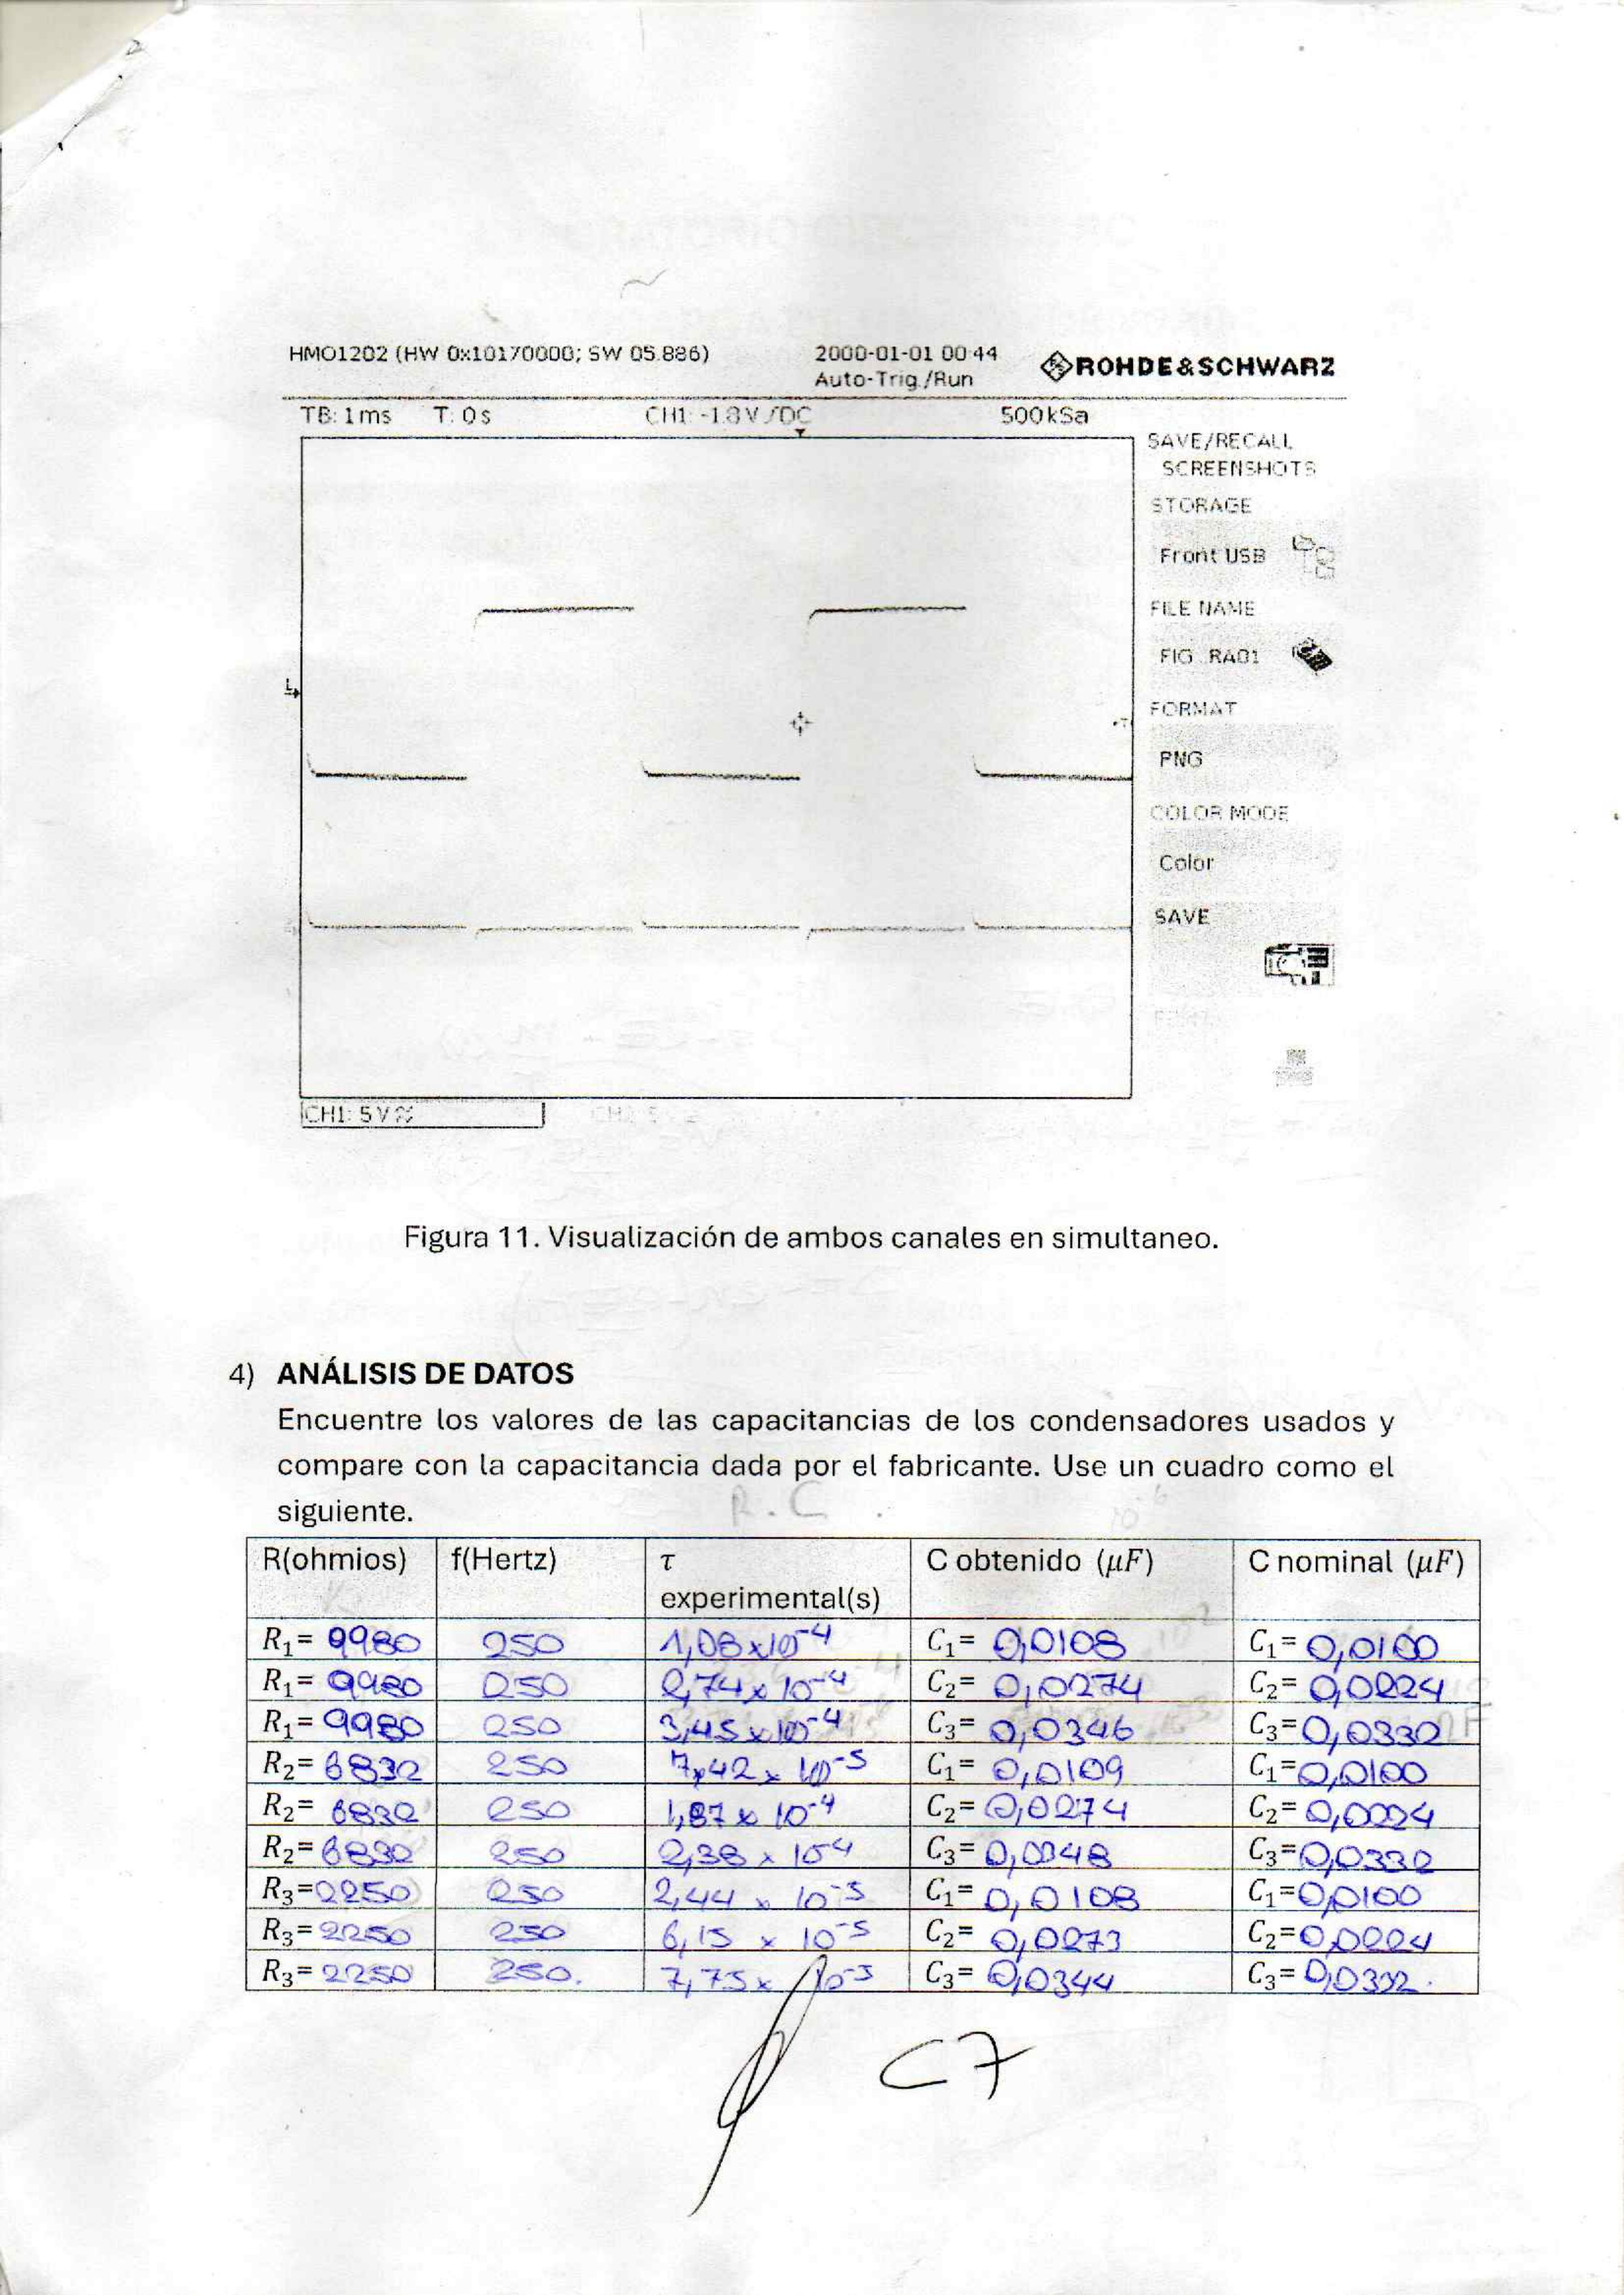
\includegraphics[width=0.75\linewidth, height=0.64\textheight, keepaspectratio]{fig_hoja_datos}
    \caption{Facsímil de la hoja de toma de datos experimentales de la Mesa C7 en el laboratorio de Física III.}
    \label{fig:hoja_datos}
\end{figure}

En dicha hoja constan los valores de calibración del generador de ondas ($f = \qty{250}{\hertz}$, $V = \qty{10,0}{\voltpp}$), las mediciones de resistencia con multímetro digital ($R_1 = \qty{9,98}{\kilo\ohm}$, $R_2 = \qty{6,832}{\kilo\ohm}$, $R_3 = \qty{2,250}{\kilo\ohm}$) y los tiempos característicos $\tau$ medidos directamente con cursores en el osciloscopio para las configuraciones ensayadas, a partir de los cuales se estructuró el análisis experimental y tratamiento metrológico del presente informe.

\end{appendices}
